\documentclass[a4paper,12pt]{article} 
\usepackage{geometry}
\usepackage{wrapfig}
\geometry{
	a4paper,
	total={170mm,257mm},
	left=10mm,
	right=10mm,
	top=20mm,
}
\usepackage{titlesec}
\titlelabel{\thetitle.\quad} %точка в section

%%% Работа с русским языком
\usepackage{cmap}                           % поиск в PDF
\usepackage{mathtext} 			 	       % русские буквы в формулах
\usepackage[T2A]{fontenc}               % кодировка
\usepackage[utf8]{inputenc}              % кодировка исходного текста
\usepackage[english,russian]{babel}  % локализация и переносы

%Математика
\usepackage{amsmath,amsfonts,amssymb,amsthm,mathtools} % AMS
\usepackage{icomma} % "Умная" запятая

%% Шрифты
\usepackage{euscript}	 % Шрифт Евклид
\usepackage{mathrsfs} % Красивый матшрифт

\usepackage{mathtext} 
\usepackage{setspace}
\usepackage{tabularx}
\usepackage{longtable}
\usepackage{icomma}
\usepackage{euscript}
\usepackage{float}
\usepackage{cutwin}
\usepackage{mathrsfs}
\usepackage{adjustbox}
\usepackage{dashbox}
\usepackage[normalem]{ulem}	
\usepackage[babel=true]{microtype}
\RequirePackage[T1]{fontenc}
\usepackage{amsmath,amsfonts,amssymb,amsthm,mathrsfs,mathtools} 
\usepackage{xcolor}         
\usepackage{enumitem}     
\usepackage{xpatch}       
\usepackage{cancel}                  
\usepackage{upgreek}                 
\usepackage{lipsum}                  
\usepackage[version=4]{mhchem}       
\usepackage{multirow}                
\usepackage{stackengine}             
\usepackage{tikz}         
\usepackage{hyperref}
\hypersetup{colorlinks=true,urlcolor=blue}       
\usetikzlibrary{positioning}         
\usepackage{titletoc}                 
\usepackage{chngcntr}              
\usepackage{fancyhdr}                
\usepackage{makecell}                
\usepackage{indentfirst}             
\usepackage{tocloft}                 
\usepackage{soul}                   
\usepackage[stable]{footmisc}       
\usepackage{subfig}                  

\mathtoolsset{showonlyrefs=true}


\theoremstyle{definition}
\newtheorem*{definition}{Определение}
\newtheorem{statement}{Предложение}[section]
\newtheorem{lemma}{Лемма}[section]
\newtheorem{theorem}{Теорема}[section]
\newtheorem*{theoremn}{Теорема}
\newtheorem*{corollary}{Следствие}
\newtheorem*{example}{Пример}
\newtheorem*{note}{Замечание}
\newtheorem*{problem}{Задача}


\counterwithout{footnote}{section}\DeclareRobustCommand{\divby}{%
	\mathrel{\text{\vbox{\baselineskip.65ex\lineskiplimit0pt\hbox{.}\hbox{.}\hbox{.}}}}%
}

\newcommand{\dotpr}[2]{\bra{#1}\ket{#2}}
\let\AA\relax
\let\emptyset\varnothing
\DeclareMathOperator*{\esssup}{ess sup}
\DeclareMathOperator*{\ord}{ord}
\DeclareMathOperator*{\supp}{supp}
\DeclareMathOperator*{\pr}{pr}
\DeclareMathOperator*{\Ker}{Ker}
\DeclareMathOperator*{\Vol}{Vol}
\DeclareMathOperator*{\rg}{rk}
\DeclareMathOperator*{\Ima}{Im}
\DeclareMathOperator*{\Alt}{Alt}
\DeclareMathOperator*{\Sym}{Sym}
\newcommand{\eqdef}{\stackrel{\text{\tiny{def}}}{=}}
\newcommand{\pp}{\partial}
\newcommand{\AA}{\mathcal{A}}
\newcommand{\BB}{\mathcal{B}}
\newcommand{\MM}{\mathbb{M}}
\newcommand{\NN}{\mathbb{N}}
\newcommand{\ZZ}{\mathbb{Z}}
\newcommand{\QQ}{\mathbb{Q}}
\newcommand{\RR}{\mathbb{R}}
\newcommand{\CC}{\mathbb{C}}
\newcommand{\FFF}{\mathbb{F}}
\newcommand{\DD}{\mathcal{D}}
\newcommand{\FF}{\mathcal{F}}
\newcommand{\sS}{\mathcal{S}}
\newcommand*\circled[1]{\tikz[baseline=(char.base)]{
		\node[shape=circle,draw,inner sep=2pt] (char) {#1};}}

%%% Заголовок
\author{Шерхалов Денис Б02-204}
\title{Лабораторная работа 3.2.4+3.2.5 \\
	\textbf{Свободные и вынужденные колебания в электрическом контуре}}
\date{\today}

\begin{document}
	
{\Large \maketitle}

\paragraph*{Цель работы:} исследование свободных и вынужденных колебаний в
колебательном контуре.
\paragraph*{В работе используются:} осциллограф АКТАКОМ ADS-6142H, генератор сигналов специальной формы АКИП-3409/4, магазин сопротивления МСР-60, магазин емкости Р5025, магазин индуктивности Р567 типа
МИСП, соединительная коробка с шунтирующей емкостью, соединительные одножильные и коаксиальные провода.

\section{Введение}
\subsection*{Экспериментальная установка} 
 Колебательный контур состоит из постоянной индуктивности $L$ с активным сопротивлением $RL$, переменной емкости C и сопротивления $R$. Картина колебаний
напряжения на емкости наблюдается на экране двухканального осциллографа. Для возбуждения затухающих колебаний используется генератор сигналов специальной
формы. Сигнал с генератора поступает через конденсатор C1 на вход колебательного контура. Данная емкость необходима чтобы выходной импеданс генератора был
много меньше импеданса колебательного контура и не влиял на процессы, проходящие в контуре. \par
Установка предназначена для исследования не только возбужденных, но и свободных колебаний в электрической цепи. При изучении свободно затухающих колебаний генератор специальных сигналов на вход колебательного контура подает периодические короткие импульсы, которые заряжают конденсатор C. За время между
последовательными импульсами происходит разрядка конденсатора через резистор
и катушку индуктивности. 
\begin{figure}[H]
    \centering
    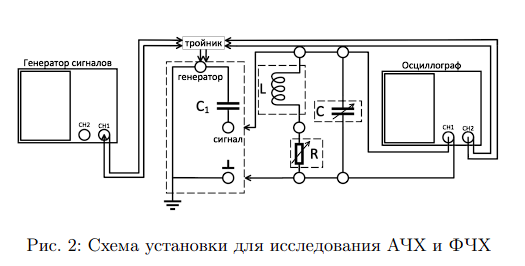
\includegraphics{2.png}    
\end{figure}
\begin{figure}[H]
    \centering
    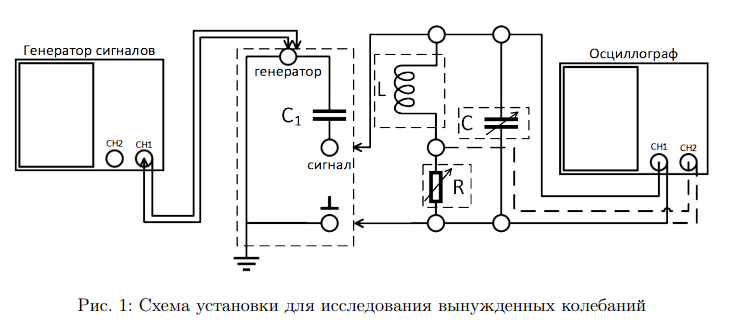
\includegraphics{1.png}    
\end{figure}

\subsection*{Теоретические сведения}

\noindent Для RLC контура применим правило Кирхгофа:
\begin{equation}
    RI + U_C + L\frac{dI}{dt} = 0.
\end{equation}
Подставив в уравнение выражение для тока через 1-ое правило Кирхгофа, и разделив обе части уравнения на $CL$, получим:
\begin{equation}
    \frac{d^2U_C}{dt^2} + \frac{R}{L} \frac{dU_C}{dt} + \frac{U_C}{CL}=0
\end{equation}
Произведём замены $\gamma = \frac{R}{2L}$ -- коэффициент затухания, $\omega_0^2 = \frac{1}{LC}$ -- собственная круговая частота, $T_0 = \frac{2\pi}{\omega_0} = 2\pi \sqrt{LC}$ -- период собственных колебаний. Тогда уравнение примет вид:
\begin{equation}
    \ddot{U_C} + 2 \gamma \dot{U_C} + \omega_0^2U_C = 0,
\end{equation}
где точкой обозначено дифференцирование по времени. Будем искать решение данного дифференциального уравнения в классе функций следующего вида:
$$U_C(t) = U(t)e^{- \gamma t}.$$
Получим:
\begin{equation}
    \ddot{U} + \omega_1^2 U = 0,
\end{equation}
где
\begin{equation}
    \omega_1^2 = \omega_0^2-\gamma^2
\end{equation}
Для случая $\gamma < \omega_0$ в силу того, что $\omega_1 > 0$, получим:
\begin{equation}
    U_C(t) = U_0 \cdot e^{-\gamma t} \text{cos}(\omega_1 t + \varphi_0).
\end{equation}
Для получения фазовой траектории представим формулу в другом виде:
\begin{equation}
    U_C(t) = e^{-\gamma t}(a \text{cos} \omega_1 t + b \text{sin} \omega_1 t),
\end{equation}
где $a$ и $b$ получаются по формулам:
$$a = U_0 \text{cos} \varphi_0, \qquad b = - U_0 \text{sin} \varphi_0.$$
В более удобном виде запишем выражения для напряжения на конденсаторе и токе через катушку:
\begin{equation}
    U_C (t) = U_{C0} \cdot e^{-\gamma t} (\text{cos} \omega_1 t + \frac{\gamma}{\omega_1} \text{sin} \omega_1 t),
\end{equation}
\begin{equation}
    I(t) = C\dot{U_C}= - \frac{U_{C0}}{\rho} \frac{\omega_0}{\omega_1} e^{-\gamma t} \text{sin} \omega_1 t.
\end{equation}
Введём некоторые характеристики колебательного движения:
\begin{equation}
    \tau = \frac{1}{\gamma} = \frac{2L}{R},
\end{equation}
где $\tau$ -- время затухания (время, за которое амплитуда колебаний уменьшается в $e$ раз).
\begin{equation}
    \Theta = \text{ln} \frac{U_k}{U_{k+1}} = \gamma T_1 = \frac{1}{N_\tau} = \frac{1}{n} \text{ln} \frac{U_k}{U_{k+n}}, 
\end{equation}
где $\Theta$ -- логарифмический декремент затухания, $U_k$ и $U_{k+1}$ -- два последовательных максимальных отклонения величины в одну сторону, $N_\tau$ -- число полных колебаний за время затухания $\tau$.

Теперь рассмотрим случай \textit{вынужденных колебаний} под действием внешней внешнего синусоидального источника. Для этого воспользуемся методом \textit{комплексных амплитуд} для схемы на рисунке (рис. 1):
\begin{equation}
    \ddot{I} + 2 \gamma \dot{I} + \omega^2 I = - \varepsilon \frac{\Omega}{L} e^{i\Omega t}.
\end{equation}
Решая данное дифференциальное уравнение получим решение:
\begin{equation}
    I = B\cdot e^{-\gamma t} \text{sin}(\omega t - \Theta) + \frac{\varepsilon_0 \Omega}{L \phi_0} \text{sin} (\Omega t - \varphi).
\end{equation}
Нетрудно видеть, что частота резонанса будет определяться формулой:
\begin{equation}
    \omega_0 = \frac{1}{2 \pi \sqrt{LC}}.
\end{equation}

Способы измерения добротности $Q = \dfrac{W_0}{W_{loss,\,\tau}} = \dfrac{\pi}{\Theta}$:
\begin{enumerate}
    \item с помощью потери амплитуды свободных колебаний: 
    \begin{equation}
        \Theta = \frac{1}{n} \text{ln}\frac{U_k}{U_{k+n}},
    \end{equation}
    \item с помощью амплитуды резонанса можно получить добротность (в координатах $U_C/U_0$, где $U_0$ -- амплитуда колебаний напряжения источника, от частоты генератора). Отсюда нетрудно определить декремент затухания $\gamma = \frac{\omega_0}{2Q}$,
    \item с помощью среза АЧХ на уровне 0.7 от максимальной амплитуды, тогда <<дисперсия>> ($\Delta \Omega$) будет численно равна коэффициенту $\gamma$, то есть $Q = \frac{\nu_0}{2 \Delta \Omega}$.
    \item с помощью нарастания амплитуд в вынужденных колебаниях:
    \begin{equation}
        \Theta = \frac{\omega_0 n}{2\text{ln} \frac{U_0 - U_k}{U_0 - U_{k+n}}}.
    \end{equation}
    \item  с помощью формулы\begin{equation}
        \Theta = \frac{1}{R}\sqrt{\frac{L}{C}}
    \end{equation}
\end{enumerate}

\section{Ход работы}
\subsection{Измерение периодов свободных колебаний}
Соберем установку с рисунка 1, выставим $R=0$ Ом, $L=100$ мГн, $C=0$ нФ,  однако контур сам по себе обладает некоторым $C_0$, благодаря которому в контуре реализуются свободные колебания \par
Измерим с помощью осцилографа период затухающих колебаний 10T = 656 мкс, по периоду колебаний вычисляем значение емкости $C_0$, по формуле
$$C_0=\frac{T^2}{4\pi^2L}=1,09\,\text{нф}$$
Изменяя емкость C проведем измерения 10 периодов \\
\begin{center}
\begin{tabular}{|c|c|c|c|c|c|c|} \hline
    $C$, нф & 1.09& 2.09 & 4.09 & 6.09& 8.09&  10.09 \\ \hline
    $T$, мкс & 65.6& 90.8&127.0 &155.1 &178.8 &199.7   \\ \hline
    $T_{theor}$, мкс & 65.6 & 90.8 & 127.1 & 155.1& 178.7 & 199.6  \\ \hline
\end{tabular}
\end{center}
\subsection{Критическое сопротивление и декремент затухания}
Рассчитаем C, при котором собственная частота колебаний $\nu=1/(2\pi \sqrt{LC})=6500$\,Гц, $C=6$\,нф. Для выбранных L и С расчитаем критическое сопротивление контура $R_{cr}=8168$\,Ом по формуле $R_{cr}=2\sqrt{L/C}$  \par
Установим на магазине емкость, близкую к расчитанной увеличивая сопротивление до критической, пронаблюдаем картину затухающих колебаний. При сопротивлении $R=6$\,кОм колебательный режим переходит в апериодический. \par
Измения сопротивление запишем зависимость логарифмического декремента от сопротивления \par
\begin{center}
    \begin{tabular}{|c|c|c|c|c|c|c|} \hline
       R,\text{Ом}  & 410& 600& 800 &1000 &1200 & 1600\\ \hline
       $U_1$ & 588 & 660 & 470 & 610 & 360 & 550  \\
       $U_2$ & 400 & 370 & 250 & 250 & 150 & 140 \\
       $U_3$ & 284 & 220 & 140 & 100 & 70 & 40  \\
       $U_4$ & 192 & 130 & --- & 40 & ---& --- \\ \hline
       $\theta$  & 0.35 & 0.54 & 0.61 & 0.91 & 0.82 & 1.31  \\ \hline
    \end{tabular}
\end{center}
\subsection{Свободное колебание на фазовой плоскости}
Проведем аналогичные измерение, но уже на фазовой плоскости и запишем результату в таблицу. \par
\begin{center}
    \begin{tabular}{|c|c|c|c|c|c|c|} \hline
       R,\text{Ом}  & 410& 600& 800 &1000 &1200 & 1600\\ \hline
       $U_1$ & 21 & 20 & 20 & 19 & 18 & 17  \\
       $U_2$ & 14 & 12 & 10 & 8 & 6 & 4 \\
       $U_3$ & 10 & 7 & 5 & 3 & 2 & 1 \\ \hline
       $\theta$  & 0.37 & 0.52 & 0.69 & 0.92 & 1.10 & 1.42  \\ \hline
    \end{tabular}
\end{center}
\subsection{Исследование резонансных кривых}
Выставим значение емкости $C = 6$ нф и сопротивление $R = 410$ Ом (на этом моменте мы вспомнили,что забыли про $C_0$ и не учитывали его в течение всей лабораторной работы, поэтому нужно пересчитать частоту, $\nu_{res}=6015$\,Гц, критическое сопротивление $R_{cr}=7511$\,Ом)\par
Изменяя частоту генератора вблизи резонансной частоты, находим резонансную частоту $\nu = 6010$ Гц и ее амплитуду $2U_{res} = 16.7$\,B. \par
Снимем АЧХ вблизи резонанса \par
\begin{center}
    \begin{tabular}{|c||c|c|c|c|c|c|c|} \hline
        $\nu$,\,Гц & 5300 & 5390& 5480 & 5570 & 5660 & 5750 & 5840\\ \hline
        $2U$,\,B & 7 & 7.8 & 8.9 & 10.2 & 11.7 & 13.7 & 15.2 \\ \hline \hline
        $\nu$,\,Гц & 5930 & 6020& 6110 & 6200 & 6290 & 6380 & 6470 \\ \hline
        $2U$,\,B & 16.4 & 16.6 & 16.2 & 15 & 13.8 & 12.6 & 11\\ \hline \hline
        $\nu$,\,Гц & 6560 & 6650 & 6740 & 6830 & 6920 & 7010 & 7100 \\ \hline
        $2U$,\,B & 10.2 & 9.4 & 8.5 & 8.1 & 7.7 & 7.1 & 6.7 \\ \hline
    \end{tabular}
\end{center}

\subsection{Обработка результатов}
\textbf{1}. Из секции 3.1 построим график $T_{exp}=f(T_{theor})$
\begin{figure}[H]
    \centering
    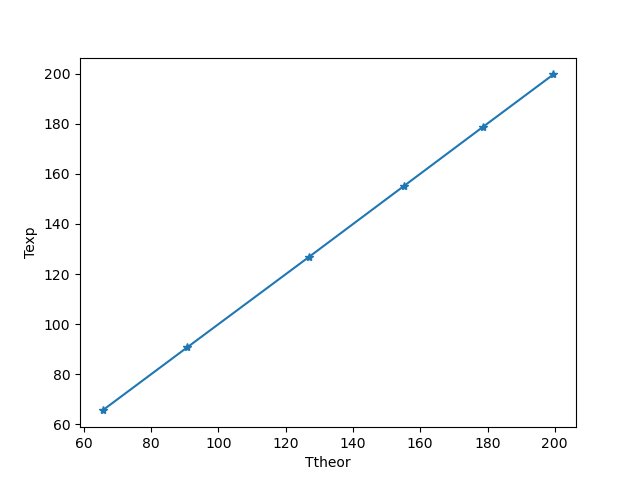
\includegraphics{324 1.png}    
\end{figure}
Из графика видно, что результаты совпали, погрешность $
<1\%$ \par
\textbf{2}.
Построим график $1/\theta^2=f[1/R^2]$
\begin{figure}[H]
    \centering
    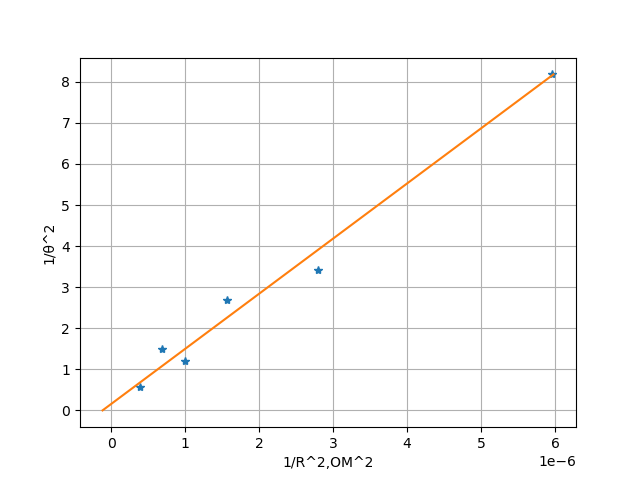
\includegraphics{324 2.png}    
\end{figure} \par
Коэффициент наклона $K=1320000 \pm 70000$\, Ом$^2$ \par
Зная коэффициент наклона, найдем $R_{cr}$, по формуле $R_{cr}=2\pi \sqrt{K}=7200 \pm 200$\,Ом, что близко с теоретическим значением $R_{cr}=7511$\,Ом \par
\textbf{3}. Расчитаем добротность для максимального и минимального значения $\theta$ и теоретическое с теми же параметрами.
\begin{itemize}
    \item Вычисление добротности контура по секции 3.2:\\
$$Q(\theta_{min})= 8.97 \qquad \qquad  Q(\theta_{max})= 2.40  $$
\item Вычисление добротности контура по секции 3.3:\\
$$Q(\theta_{min})= 8.49 \qquad \qquad  Q(\theta_{max})= 2.21  $$
    \item Вычисление добротности контура теоретически:\\   
$$Q(\theta_{min})= 9.16 \qquad \qquad  Q(\theta_{max})= 2.34  $$
\end{itemize}
\textbf{4}. По секции 3.4 построим АЧХ в масштабе $U/U_{res}=f(\nu /\nu_{res})$
\begin{figure}[H]
    \centering
    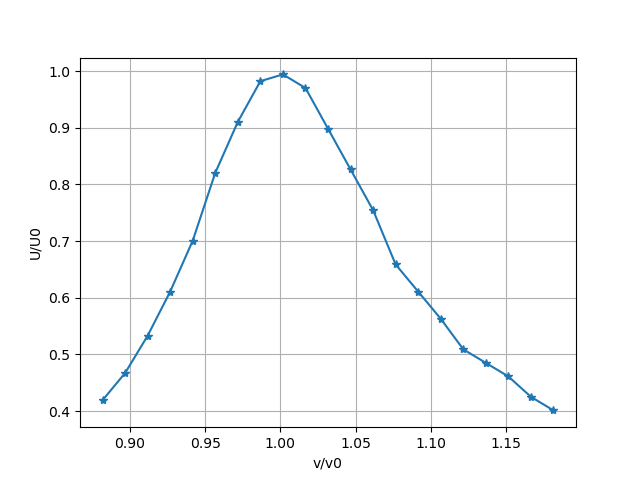
\includegraphics{324 3.png}    
\end{figure} \par
\textbf{5}. Рассчитаем добротность по формуле $Q=\nu_{res}/2\Delta \Omega$, Q=7.91
\section{Вывод}
\begin{enumerate}
    \item С учетом емкости системы, значения периодов эксперимента идеально совпали с теоретическими значениями периодов.
    \item Удалось снять зависимость логарифмического декремента затухания от активного сопротивления цепи (погрешность составила порядка $5\%$)
    \item Определили критическое сопротивление, при котором характер колебаний меняется на апериодический, тремя способами: теоретическим $R_{кр} = 7.5$\,кОм, по наклону графика зависимости логарифмического декремента затухания от сопротивления цепи $R_\text{кр} = 7.2 \pm 0,2 \ \text{кОм},$ с помощью наблюдением за картиной колебаний $R_\text{кр} = 6 \ \text{кОм}.$ 
    \item Результаты расчетов добротности сведены в таблицу: \\
    \begin{center}
        \begin{tabular}{|c|c|c|c|c|c|c|c|} \hline
             &\multicolumn{3}{c}{Свободные колебания} &\multicolumn{4}{|c|}{Вынужденные колебания} \\ \hline{}
           R, Ом & f(LCR) & f($\nu$) & Спираль& АЧХ & ФЧХ & Нарастание & Затухание\\ \hline
          410 &9.16 & 8.97& 8.49 & 7.91 & -& -&- \\ \hline
          1600 & 2.34 & 2.4& 2.21 & - & -& -&- \\ \hline
        \end{tabular}
            
    \end{center}

 Как видим, все добротности хорошо совпали.

\end{enumerate}


\end{document}